%% This is file `elsarticle-template-1-num.tex',
%%
%% Copyright 2009 Elsevier Ltd
%%
%% This file is part of the 'Elsarticle Bundle'.
%% ---------------------------------------------
%%
%% It may be distributed under the conditions of the LaTeX Project Public
%% License, either version 1.2 of this license or (at your option) any
%% later version.  The latest version of this license is in
%%    http://www.latex-project.org/lppl.txt
%% and version 1.2 or later is part of all distributions of LaTeX
%% version 1999/12/01 or later.
%%
%% Template article for Elsevier's document class `elsarticle'
%% with numbered style bibliographic references
%%
%% $Id: elsarticle-template-1-num.tex 149 2009-10-08 05:01:15Z rishi $
%% $URL: http://lenova.river-valley.com/svn/elsbst/trunk/elsarticle-template-1-num.tex $
%%
\documentclass[preprint,12pt]{elsarticle}

%% Use the option review to obtain double line spacing
%% \documentclass[preprint,review,12pt]{elsarticle}

%% Use the options 1p,twocolumn; 3p; 3p,twocolumn; 5p; or 5p,twocolumn
%% for a journal layout:
%% \documentclass[final,1p,times]{elsarticle}
%% \documentclass[final,1p,times,twocolumn]{elsarticle}
%% \documentclass[final,3p,times]{elsarticle}
%% \documentclass[final,3p,times,twocolumn]{elsarticle}
%% \documentclass[final,5p,times]{elsarticle}
%% \documentclass[final,5p,times,twocolumn]{elsarticle}

%% The graphicx package provides the includegraphics command.
\usepackage{graphicx}
\graphicspath{ {./images/} }
%% The amssymb package provides various useful mathematical symbols
\usepackage{amssymb}
\usepackage{amsmath}
%% The amsthm package provides extended theorem environments
%% \usepackage{amsthm}

%% The lineno packages adds line numbers. Start line numbering with
%% \begin{linenumbers}, end it with \end{linenumbers}. Or switch it on
%% for the whole article with \linenumbers after \end{frontmatter}.
\usepackage{lineno}

%% natbib.sty is loaded by default. However, natbib options can be
%% provided with \biboptions{...} command. Following options are
%% valid:

%%   round  -  round parentheses are used (default)
%%   square -  square brackets are used   [option]
%%   curly  -  curly braces are used      {option}
%%   angle  -  angle brackets are used    <option>
%%   semicolon  -  multiple citations separated by semi-colon
%%   colon  - same as semicolon, an earlier confusion
%%   comma  -  separated by comma
%%   numbers-  selects numerical citations
%%   super  -  numerical citations as superscripts
%%   sort   -  sorts multiple citations according to order in ref. list
%%   sort&compress   -  like sort, but also compresses numerical citations
%%   compress - compresses without sorting
%%
%% \biboptions{comma,round}

% \biboptions{}

\usepackage[utf8]{inputenc}
\usepackage[english]{babel}
%%\usepackage[demo]{graphicx}
%%\usepackage{babel,blindtext} 

\usepackage{xcolor}

\journal{Journal Name}

\begin{document}

\begin{frontmatter}

%% Title, authors and addresses

\title{Proteinas Canijas}

%% use the tnoteref command within \title for footnotes;
%% use the tnotetext command for the associated footnote;
%% use the fnref command within \author or \address for footnotes;
%% use the fntext command for the associated footnote;
%% use the corref command within \author for corresponding author footnotes;
%% use the cortext command for the associated footnote;
%% use the ead command for the email address,
%% and the form \ead[url] for the home page:
%%
%% \title{Title\tnoteref{label1}}
%% \tnotetext[label1]{}
%% \author{Name\corref{cor1}\fnref{label2}}
%% \ead{email address}
%% \ead[url]{home page}
%% \fntext[label2]{}
%% \cortext[cor1]{}
%% \address{Address\fnref{label3}}
%% \fntext[label3]{}


%% use optional labels to link authors explicitly to addresses:
%% \author[label1,label2]{<author name>}
%% \address[label1]{<address>}
%% \address[label2]{<address>}

\author[1]{Ale Zavala}
\author[1]{Sergio Hern\'andez }
\author[1]{Pedro Miramontes}
\author[2]{León Martínez}

\address[1]{Facultad de Ciencias, National Autonomous University of Mexico, Mexico City 04510, Mexico}
\address[2]{Metropolitan Autonomous University}

\begin{abstract}
%% Text of abstract
¿Qué proponemos como abstract?
\end{abstract}

\begin{keyword}
Intrinsically disordered protein regions \sep protein structure \sep family \sep domain \sep DGBD
%% keywords here, in the form: keyword \sep keyword

%% MSC codes here, in the form: \MSC code \sep code
%% or \MSC[2008] code \sep code (2000 is the default)

\end{keyword}

\end{frontmatter}

%%
%% Start line numbering here if you want
%%
\linenumbers

%% main text
\section{Background}
\label{S:1}




Historically, the science of protein structure has privileged the study of ordered protein regions (OPRs)  with regular and well-defined secondary structure, such as  $\alpha$-helix, $\beta$-conformations and turns. In fact, proteins that contain mainly ordered regions are the classic text-book example of what a typical protein should look like. This is probably associated with the fact that the most commonly used technique for determining protein structure, i. e. x-ray crystallography, is biased towards resolving protein regions with regular and well-defined secondary structures. However,  it has recently become increasingly clear that intrinsically disordered protein regions play an important role in the structure of proteins \cite{oldfield2014intrinsically}.

Intrinsically disordered protein regions (IDPRs), are segments of polypeptides, that do not natively acquire well defined, regular, or repetitive, secondary structures and instead adopt many different structural ensembles with no single, preferred lowest energy conformation and have biological activities that are dependent on this disordered state. There are some computational tools that can predict the order/disorder state of a protein region using only the complete polypeptide sequence as input \cite{vucetic2004disprot},  \cite{piovesan2016disprot}. IDPRs have been found to be prevalent in eukaryotes and are common in bacteria and archaea too (XXX?  ¿PEDRO: que significa esta nota?)  \cite{dunker2000intrinsic} \cite{dunker2002intrinsic} \cite{dunker2013s} \cite{oldfield2014intrinsically}. A general function that has been proposed for many IDPRs is the binding to other molecules, including proteins, nucleic acids and other ligands \cite{dunker2001intrinsically} \cite{van2014classification} \cite{oldfield2014intrinsically}. However, it is possible that the importance of IDPRs goes beyond this currently accepted function, and that they may even play an important role in the folding and functioning of proteins. We would like to emphasize that in this study we have tried to jointly analyze both the OPRs and IDPRs. This approach derives from our belief that at least some of the properties of proteins are the product of the interactions between OPRs and IDPRs. Furthermore, we hypothesize that the distribution pattern of OPRs and IDPRs within a given protein domain is specific to that domain  (similar to a fingerprint) and also specific to that domain’s family. We will expand on the definition of protein families and other related concepts in the following sections. 

HERE, WE WILL ONLY MENTION THAT STUDYING PATTERNS OF PROTEIN ORDER/DISORDER AT THE LEVEL PROTEIN DOMAINS (INSTEAD OF SINGLE PROTEINS) ALLOWED US TO CAPTURE  AMINO ACID SEQUENCE VARIABILITY  THAT WAS, IN PRINCIPLE, COMPATIBLE WITH THE TERTIARY STRUCTURE CONSERVATION THAT CHARACTERIZES A DOMAIN. ADDITIONALLY,  EACH REPRESENTATIVE OF A DOMAIN ACTED AS A NEW QUASI-REPLICATE THEREOF, ALLOWING US TO (NATURALLY) INCREASE THE SAMPLE SIZE OF THE DATA SERIES TO BE ANALYZED WITH OUR PROPOSED STATISTICAL TOOLS (SEE BELOW). FURTHERMORE, WE AUGMENTED OUR PROTEIN SEQUENCE DATA WITH GENE ONTOLOGY (GO) ANNOTATIONS IN ORDER TO EXPLORE WHETHER FUNCTIONAL INFORMATION OF PROTEIN DOMAINS CORRELATES WITH  THEIR ORDER/DISORDER REGULARITIES.

Measures of complexity of patterns of OPRs and IDPRs have the potential to contain information on structural and functional aspects of proteins in the sense that members of a given protein family that are close to each other in the parameter space of some measures of complexity could also be close in terms of functional properties. If IDPRs are an integral part of proteins the patterns of alternating OPRs and IDPRs of varying lengths should be relatively conserved among members of a protein family. Potentially, measures of the complexity of such patterns could capture enough information thereof, such that they could serve as a proxy for characterizing specific proteins.

In this study we will use several measures of complexity of a polypeptide pattern. At this time "complexity" can be understood as how close or how far a sequences is from two extremes: randomness or periodicity. On one hand, he well known Kolmogorov’s complexity index (K) provides a measure of how far a sequence is from being random and, on the other,  Shannon’s entropy (H) tells us how far is a sequence from the equiprobable distribution (REFSXXX). Additionally, the recently proposed Discrete Generalized Beta function (DGBF)  of rank-ordered distributions has also emerged as a measure of complexity. INTERESTINGLY, THE DGBF CAN SEPARATE INTERMITTENT REGIMES FROM CHAOTIC DYNAMICS AND MAY SERVE AS AN INDICATOR OF TRANSITIONS BETWEEN THESE TWO REGIMES IN A WIDE ARRAY OF PHENOMENA  \cite{martinez2009universalit}.

Here, we propose  the use of the above mentioned descriptors to place any given protein into a space of parameters and to discuss they way different families of proteins group in such a space. Our working model will be the Saccharomyces cerevisae proteome. WE DISCUSS THE POSSIBILITY THAT THE DGBF OF PATTERNS OF PROTEIN ORDER/DISORDER MAY BE ABLE TO DETECT EVOLUTIONARY TRANSITIONS IN WHICH ORDERED PROTEINS ACQUIRE OR EXPAND THEIR DISORDERED REGIONS OR IN WHICH DISORDERED PROTEINS START TO LIMIT THEIR CONFORMATIONAL REPERTOIRES.



\bigbreak



\section{Materials and Methods}
\label{S:1}

\subsection{Construction of the database of complete sequences represented in the yeast familiome}

In this study, our aim is to characterize protein families in terms of the entropy, algorithmic complexity and characteristic beta function of their order-disorder pattern. A family of proteins is  a group of proteins or  protein domains that share patterns of significant sequence conservation, due to common ancestry, that frequently entail functional similarity \cite{nelson2017lehninger}. A protein domain is a substructure produced by any contiguous part of a polypeptide chain whose structural features are independent of the rest of the protein. A domain usually contains between 40 to 350 amino acids, and it is the modular unit from which many larger proteins are constructed \cite{alberts2015molecular}. It is important to note that any given protein does not necessarily belong to a single family, as a given protein can contain several domains with different evolutionary histories, and indeed, many proteins belong to several families \cite{bateman1999pfam}. Although most protein domains that are identified using sequence-based approaches are have well-defined and relatively stable spatial structures, some can be fully or largely disordered or can contain conserved disordered regions \cite{xue2010pondr}, these are known as intrinsically disordered domains (IDDs; \cite{tompa2009close}).
The protein families information is provided by the Pfam database \citet{sonnhammer1997pfam} \cite{bateman2004pfam} \cite{punta2011pfam} \cite{finn2015pfam}. Pfam is a collection of protein domains and protein families in which each family is represented by two multiple sequence aligments and two profile-Hidden Markov Models, one of the two alignments is a high quality seed alignment \cite{sonnhammer1997pfam} \cite{bateman2004pfam}.
To build our yeast familiome database, we explored protein information in several biological databases. To every translated gene from Saccharomyces Genome Database (“PROTEINS.txt” file, v2015; https://www.yeastgenome.org/; \cite{cherry2012saccharomyces}) we associated an UniProt identifier and its complete polypeptide sequence (“uniprot” full file, v2014; \cite{gene2015gene}). Using the UniProt information, we linked to every yeast protein its corresponding  Pfam families (“pfam-A.full”, “pfamseq” and “Pfam-A.fasta”, v28, 2015; https://pfam.xfam.org/;  \cite{bateman1999pfam}  \cite{punta2011pfam}). Subsequently, for each Pfam family from S. cerevisiae familiome we downloaded its Pfam-A seed alignment file (v28, 2015; \cite{sonnhammer1997pfam} \cite{punta2011pfam} (XXXXXXXX ?) , which contains only the aligned segments that belong to a protein family of a variety of species. Finally, we used the UniProt identifier provided by the Pfam-A seed alignment file and the UniProt full file to obtain the complete polypeptide sequence of each protein in the Pfam-A seed alignments of the yeast familiome. 


\subsection{Predicting intrinsically disordered residues in each polypeptide sequence of yeast familiome}

In order to assign each residue from our complete polypeptide sequence yeast familiome database to either the “ordered” or “intrinsically disordered” categories we used the open-source DisEMBL prediction software. DisEMBL is  based on artificial neural networks trained to predict three different definitions of disorder and displays  the disordered segments of arbitrary length within a protein sequence \cite{linding2003protein}. We used the three differents algorithms of DisEMBL: loops/coils, hot loops and remark465 and the final assignment of each residue as either ordered  or  disordered residue  was based on a majority rule decision between the three predictions. The order/disorder information was coded into the sequences as UPPERCASE/lowercase one-letter amino acid symbols, respectively. This procedure was performed for each complete polypeptide sequence of each Pfam-A seed alignment family in the yeast familiome. All the members in one family were concatenated together into one big megasequence.
 

\subsection{Transferring the ordered/disordered information to the Pfam-A families seed alignment}

In our study, we needed to associate sequences of the Pfam-A families seed alignment of the yeast familiome with the DisEMBL majority rule decision results. In order to do this we used options of the MAFFT program to maintain the Pfam-A families seed alignment unchanged, to maintain the gaps, the UPPERCASE/lowercase in the alignment and to preserve intact the order of the residues \cite{katoh2012adding} \cite{katoh2012adding} in the Pfam-A families seed alignment of the yeast familiome. 


\subsection{Gene Ontology annotations in the yeast familiome}

To enrich our yeast familiome database, for those Pfam families where this information was available, we associated the molecular function annotation from Gene Ontology (GO; ``pfam\_gene\_ontology.txt" file; v2018; http://geneontology.org/; \cite{ashburner2000gene} \cite{gene2015gene}). We needed a general molecular function annotation so we manually curated the specific GO molecular function annotations of the yeast familiome. 


\subsection{Megasequence construction}
In order to have a sequence big enough to statistically represent the whole family, we constructed what we called a megasequence which consisted in all the primary sequences (domain sequence?) for each protein within the family glued together, so the statistical regularities will be magnified and easily observable in the so called megasequence.

We took all the aligned sequences and merge them together one after another to make a family megasequence.

\subsection{The discrete generalized beta distribution (DGBD)}

All these megasequences of the yeast familiome were compared using a discrete generalized beta distribution (DGBD) \cite{martinez2009universality} \cite{petersen2011statistical} which is a rank ordering distribution that takes the form:

\begin{equation}
f(r) = \dfrac{A(N+1-r)b}{r^a}  
\end{equation}

Where a and b are parameters to be found, N is the number of ranks and A is a normalization constant. This rank ordering distribution has been successfully used across a wide range of different phenomena regardless of the truncated scaling behavior shown typically in most of the rank-order distributions.
The approach used in our analysis is as follows. We took all the aligned sequences and merge them together one after another to make a family megasequence, then we counted the frequencies of the different words of length 2 and ordered these distributions of sizes in decreasing order. Then, through a nonlinear fit of (1) we obtained the (a,b) pair which was used to represent the distribution. 

\subsection{Shannon Entropy (H(X))}
Another attribute added to the whole yeast familiome was the calculation of Shannon’s Entropy for each of the sequences of the larger. Shannon’s Entropy is defined as follows:

\[
H(X) = \sum(p\_i/log(p\_i))      (2)
\]

Where p\_i is the probability of one of the N amino acids in the megasequence X. Applying H(X) to every family megasequence we have will reveal which sequences are the furthest from the normal distribution and so, which megasequence has the most structure in it (Adami, 2004).

\subsection{Kolmogorov complexity}

Kolmogorov complexity index when applied to a string of characters, in our case is the megasequence X, can be interpreted as the complexity of a computer program required to reproduce megasequence X. The calculation of Kolmogorov’s complexity index can be approximated as follows:

\[
K(seq) =  length(compressed(seq)) /  length(seq)	(3)
\]

Where seq is the original megasequence of some family of proteins. The actual implementation of this function was done in Python computer language where zlib libraries were used to compress every sequence of the familiome (Li \& Vianyi, 2008) 
In our experiment we used K as another attribute together with the already described, in order to understand the algorithmic complexity assumed to exist in every family. That is, if a set of instructions is behind the description of every protein in each family, we would expect that K captures this particular complexity.


\subsection{SOM}

The self-organizing map is an unsupervised neural network used for data analysis and dimensionality reduction (Kohonen, 2013). It has been long being applied into data analysis and biological sciences to detect similar profiles of analyzed data (Wang et al 2002; Carlberg, Neme et al 2018... ). The basic algorithm is divided in two steps. First, an initial map is formed with N neurons arranged in a lattice which will represent M d-dimensional vectors. Each of the N neurons contains a single d-dimensional prototype that will be modified during the training of the map. Then, for each vector sample a winning prototype must be found. The second step consists in modifying the prototypes of all vectors within a neighborhood of this winning neuron, the magnitude of the modification is in proportion to the distance of the winning neuron. This process ends up unfolding a map where each prototype in neurons represents local averages of data, hence nearby neurons have similar prototypes.
Once the SOM is formed, locally grouped families must be assigned to a group. This step is done by a hierarchical clustering using euclidean distance. The number of groups was determined by the Davies-Bouldin index.


\section{Results}
\label{S:1}

\subsection{Saccharomyces cerevisiae familiome database}

Our Saccharomyces cerevisiae familiome database has 538 Pfam families and 85062 domains sequences and its full amino acid residue from each protein sequence and 82219  amino acid disordered residues added to the Pfam-A families seed alignment with 260 Pfam families with GO molecular function annotation.

\subsection{Using a discrete version of the generalized beta function to classified {\it S. cerevisiae} familiome}


\begin{figure} %{\textwidth}
    \centering
    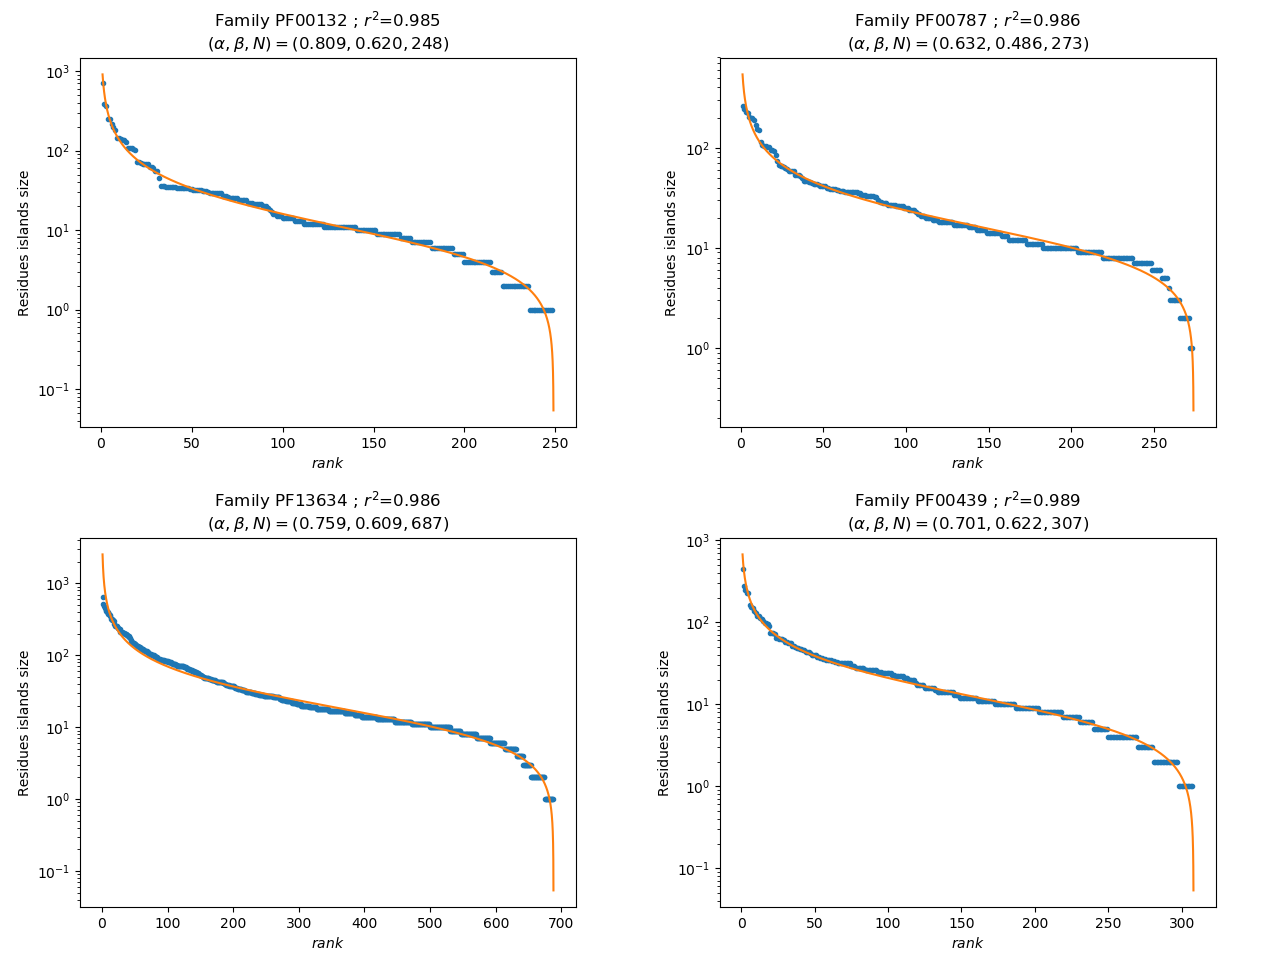
\includegraphics[width=15cm]{images/01_mejoresAlfa.png}
    \caption{Semilog DGBD plots with high alpha and low beta values. PF00787 and PF00439 families have binding molecular function ontology. PF00132 and PF13634 do not. Notice that the scales are different.}
    \label{fig:alpha}
\end{figure}
\bigbreak
Out of the best 30 DGBD graphs with high alpha and low beta values, there are 12 different ontologies belonging to 11 different families. Seven from these eleven have binding ontology, 2 have ligase ontology. Oxidoreductase, isomerase and lyase ontologies have one each.


\begin{figure} %{\textwidth}
    \centering
    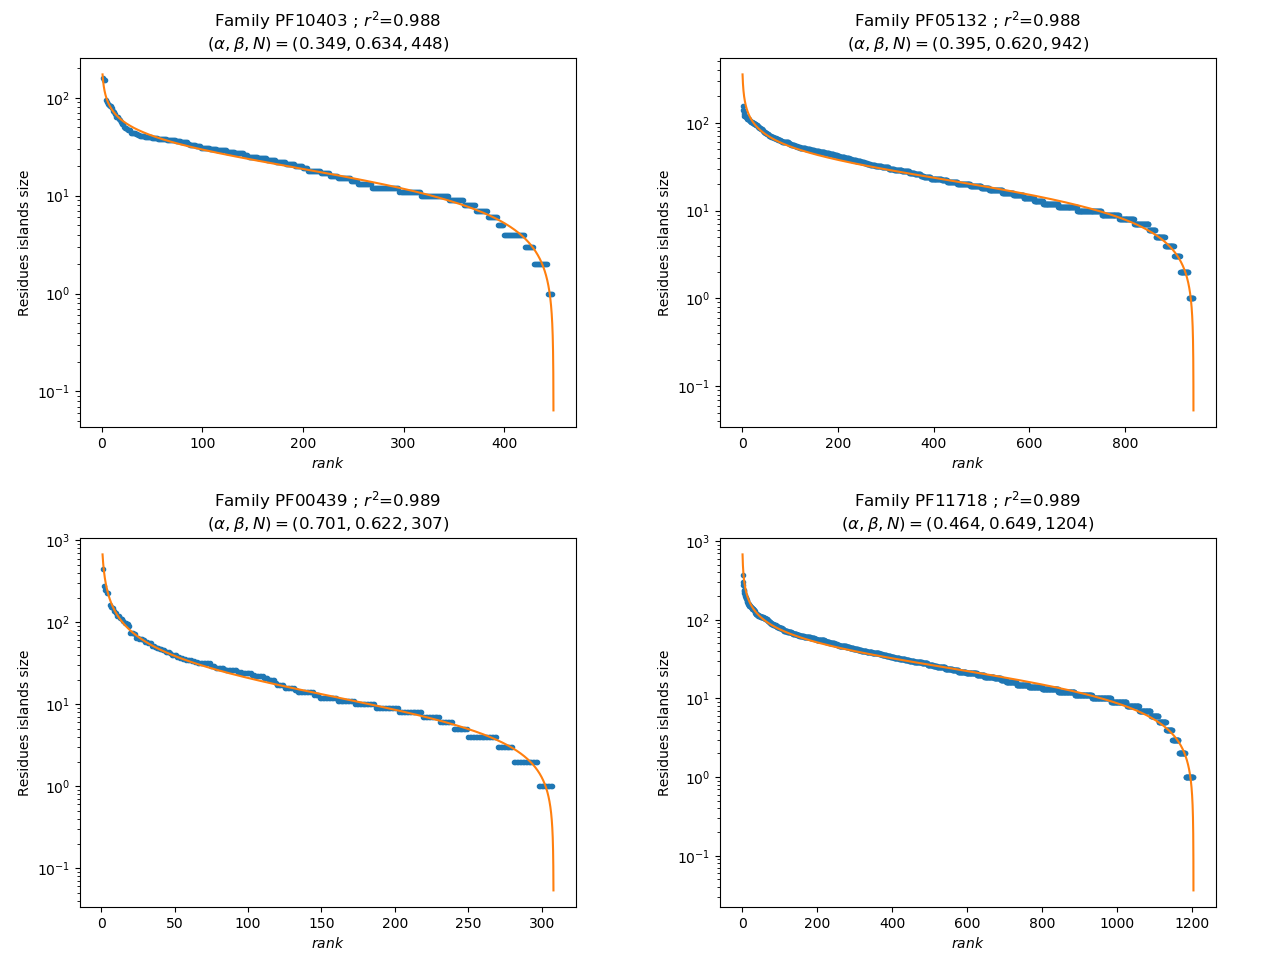
\includegraphics[width=15cm]{images/02_mejoresBeta.png}
    \bigbreak
    \caption {Semilog DGBD plots with high beta and low alpha values. PF05132 family has transferase and binding ontology. PF00439 and PF10403 share binding ontology. Notice that the scales are different.}
    \label{fig:beta}
\end{figure}
\bigbreak
Out of the best 30 DGBD graphs with high alpha and low beta values, there are 12 different ontologies. Seven families have binding ontology. Transferase, translocase and ligase have just one. It is clear the binding function prevalence.


\begin{figure} %{\textwidth}
    \centering
    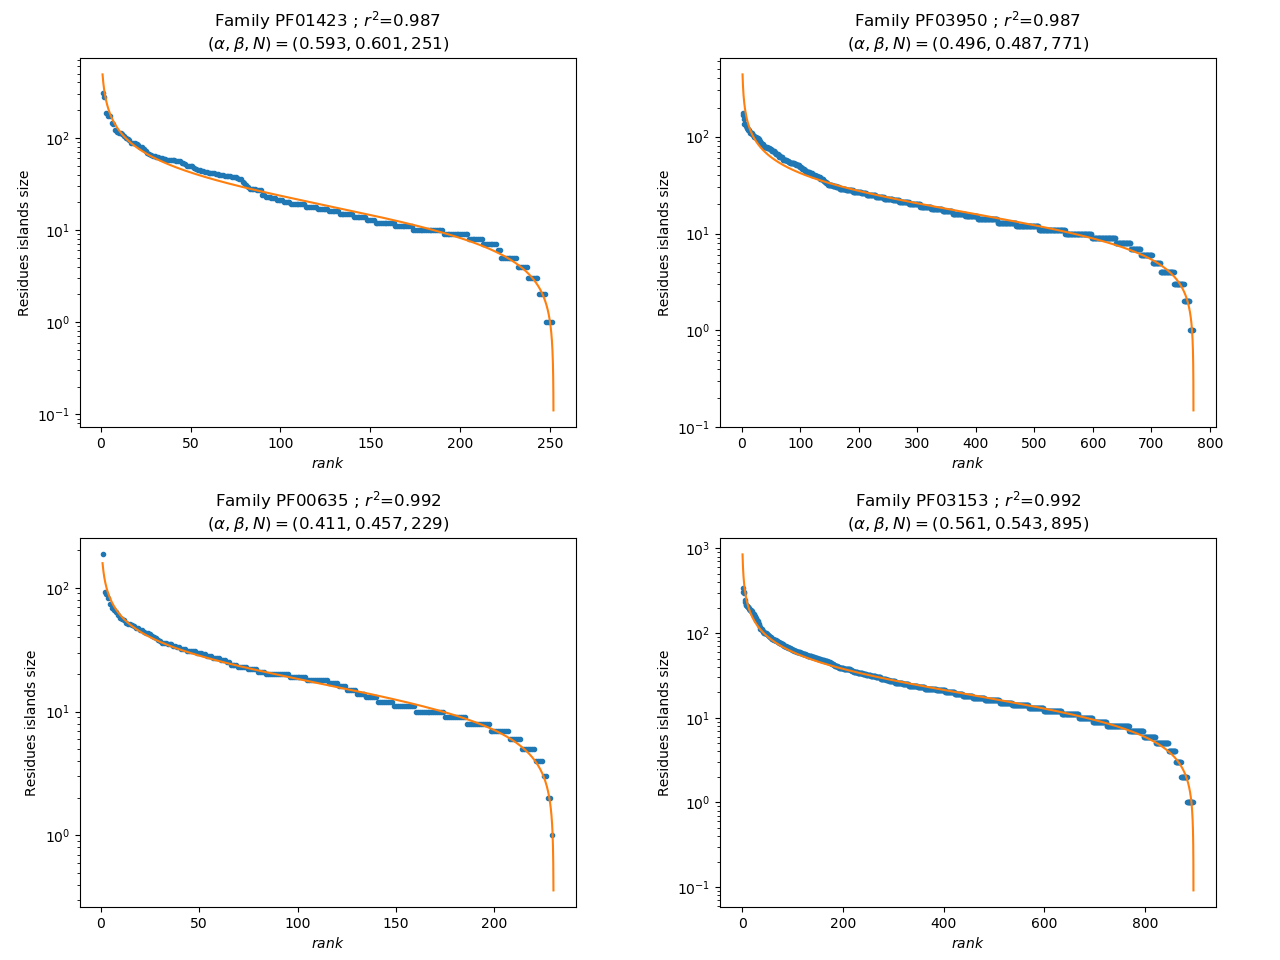
\includegraphics[width=15cm]{images/03_mejoresLaVallete.png}
    \bigbreak
    \caption {Semilog DGBD plots when alpha equals beta. PF03950 has binding and initiating factor ontologies. The scales are different.}
    \label{fig:alphabeta}
\end{figure}
\bigbreak
28 different families were found when alpha equals beta. 9 have molecular function ontologies, six have binding ontology, two have ligase ontologies. Hydrolase, initiation factor and cooper chaperone ontologies are represented by one each.



\subsection{\textbf{Self-organizing map.}}

In this work we use a self-organizing map with input data from in a 7-dimensional space. Three variables correspond to gene ontology features such as binding, transferase and hydrolase, which are coded in a binary variable whether the attribute is in the family or not. The other four features are: parameters a and b from expression (1),  Shannon’s entropy and Kolmogorv complexity.

The map was trained with a lattice of 14x14 units. In figure 7a we can see the final map where we can detect 6 groups of families located in the darker blue areas, and in 7b we can see in a heatmap each one of different entries of the prototypes, this visualization allows us to see the distribution of the different attributes. In this map all of the 7 attributes were used.
From this final figure we can infer that the gene ontology attributes are completely independent from each other. 


\begin{figure}
\minipage{0.5\textwidth}
  \includegraphics[width=\linewidth]{images/01_SOM.jpg}
  %%\caption{SOM}
  \label{fig:som}
\endminipage\hfill
\minipage{0.5\textwidth}
  \includegraphics[width=\linewidth]{images/02_SOM.jpg}
  %%\caption{HeatMap}
  \label{fig:heatmap}
\endminipage
\caption{Self organized map of the whole familiome with all of the selected features. The first four are the a, b, H and K, and the last three are the gene ontology functions associated with each family. }
\end{figure}

\bigbreak
These patterns and groups shown in figure 4 cannot be formed neither using gene ontologies  nor the complexity features alone. This can be seen in figure 5 and 6 where two maps were constructed using the before mentioned groups of features respectively.  As shown in both of these figures, the lack of a more complex structure like the one shown in figure 4 gives an idea of how the conjunction of both sets of features is required to accomplish such rich structure.

\bigbreak

\begin{figure}
\minipage{0.3\textwidth}
  \includegraphics[width=\linewidth]{images/03_SOMgo.jpg}
  %%\caption{SOM}
  \label{fig:som}
\endminipage\hfill
\minipage{0.3\textwidth}
  \includegraphics[width=\linewidth]{images/04_SOMatributos_K_H_a_b.jpg}
  %%\caption{HeatMap}
  \label{fig:heatmap}
\endminipage\hfill
\minipage{0.3\textwidth}
  \includegraphics[width=\linewidth]{images/05_SOMalfaBeta.jpg}
  %%\caption{HeatMap}
  \label{fig:heatmap}
\endminipage
\caption{a) SOM only with gene ontology features. b) SOM only with complexity features (H and K). c) SOM only with alpha and beta.}
\end{figure}


\bigbreak


\section{\textbf{Conclusions.}}
\label{S:1}

\bigbreak


\section{\textbf{References.}}
\label{S:1}

%% The Appendices part is started with the command \appendix;
%% appendix sections are then done as normal sections
%% \appendix

%% \section{}
%% \label{}


%% Following citation commands can be used in the body text:
%% Usage of \cite is as follows:
%%   \cite{key}          ==>>  [#]
%%   \cite[chap. 2]{key} ==>>  [#, chap. 2]
%%   \citet{key}         ==>>  Author [#]

%% References with bibTeX database:

% \bibliographystyle{model1-num-names}

%% New version of the num-names style
\bibliographystyle{elsarticle-num-names}
\bibliography{sample.bib}


%% Authors are advised to submit their bibtex database files. They are
%% requested to list a bibtex style file in the manuscript if they do
%% not want to use model1-num-names.bst.

%% References without bibTeX database:

% \begin{thebibliography}{00}

%% \bibitem must have the following form:
%%   \bibitem{key}...
%%

% \bibitem{}

% \end{thebibliography}


\end{document}

%%
%% End of file `elsarticle-template-1-num.tex'.
